\section{What if the US had pursued fiscal consolidation during the Great Recession?}


\subsection{A Reductions in Government Transfers in 2010}

During The Great Recession, while the US pursued fiscal stimulus, European countries engaged in large fiscal consolidations. These austerity measures led to large contractions in GDP \citep{Jorda2016,FATAS2018,House2020}. Further, unemployment scarring has been shown to be very much present, and slightly worse, in Europe.\footnote{\cite{Bertheau2023} } In this section, I consider the path of the US economy had it engaged in similar austerity measures. I augment the simulation in the previous section by simulating a counterfactual where the US reduces government spending by $2\%$ of GDP at the beginning of 2010. I assume the shock has a quarterly persistence of 0.9 such that its path fades by 2016. As in the Great Recession simulation, the tax rate cannot adjust for 10 years and set $\phi_{b}=0.015$. To account for the zero lower bound, I set the the coefficients of the Taylor rule on output, $\phi_{Y}$, and inflation, $\phi_{\pi}$, to zero such that the central bank fixes the nominal rate in response to this shock. I augment the estimated demand and monetary policy shocks from the previous section with this fiscal consolidation shock and simulate the path of the economy. Figure \ref{FC_US} plots the deviation in government spending, GDP, debt to GDP, and debt in the baseline simulation (purple), the simulation with fiscal consolidation (red), and the path of these aggregates without human capital losses (green dashed). In figure \ref{FC_US}, fiscal consolidation causes a persistent decline in GDP while only generating a slight decline a debt and debt to GDP. In particular, the decrease in government spending of  $2\%$ of GDP only decreases debt to GDP by $1$ percentage point. In the absence of human capital losses from scarring, the green dashed line demonstrates that debt to GDP would have fallen by $2.4$ percentage points. Overall, fiscal consolidation during the Great Recession would have generated a large and persistent decline in GDP while being ineffective at reducing debt to GDP.


\begin{figure}[t!] % "[t!]" placement specifier just for this example
\centering
\begin{minipage}{0.51\textwidth}
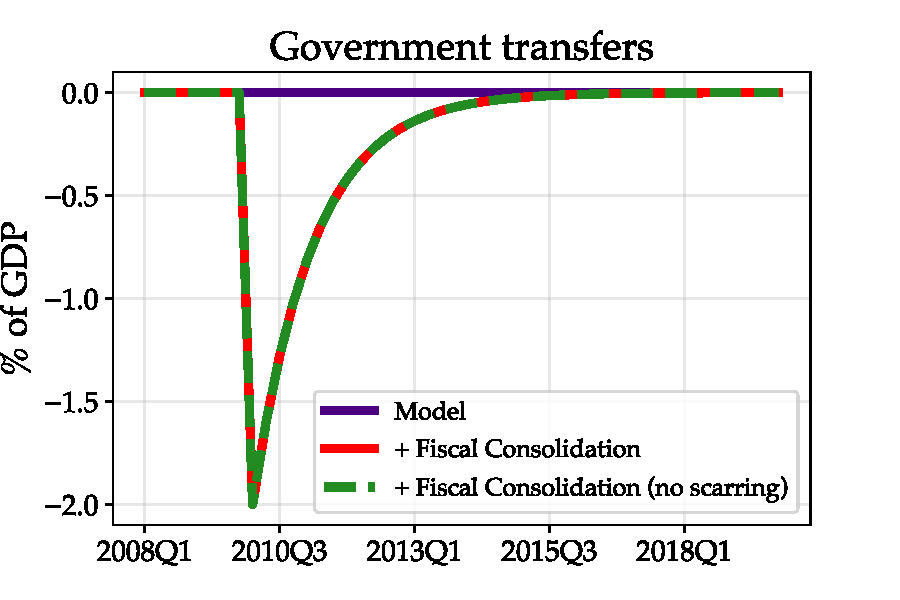
\includegraphics[scale=.57]{text/chapter1/Figures/Fiscal_Consolidation_CounterFactual/transfer_shocks_fiscal_consolidation}
 \label{fig:a}
\end{minipage}\hspace*{\fill}
\begin{minipage}{0.51\textwidth}
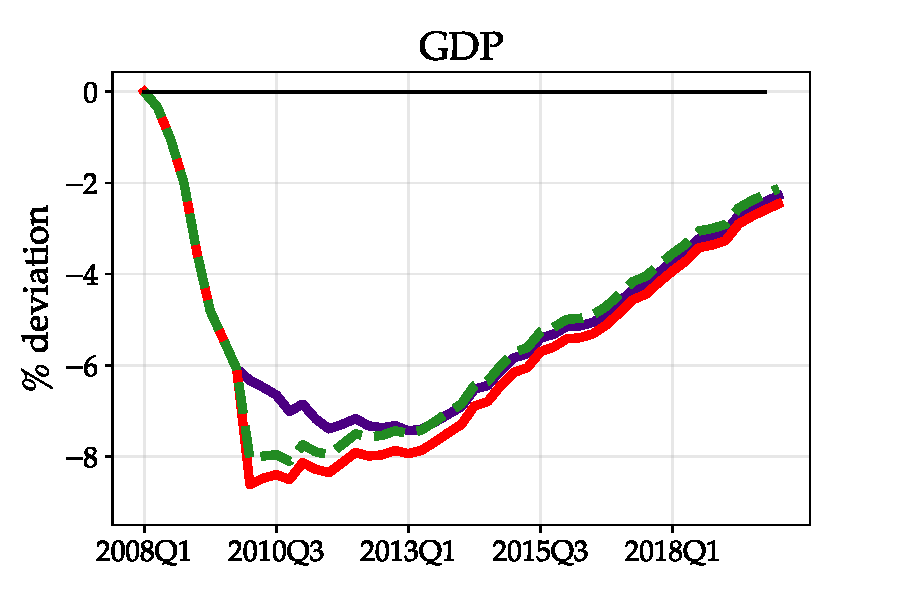
\includegraphics[scale=.57]{text/chapter1/Figures/Fiscal_Consolidation_CounterFactual/GDP_CounterFactual_Fiscal_Consolidation}
 \label{fig:b}
\end{minipage}

\medskip
\begin{minipage}{0.51\textwidth}
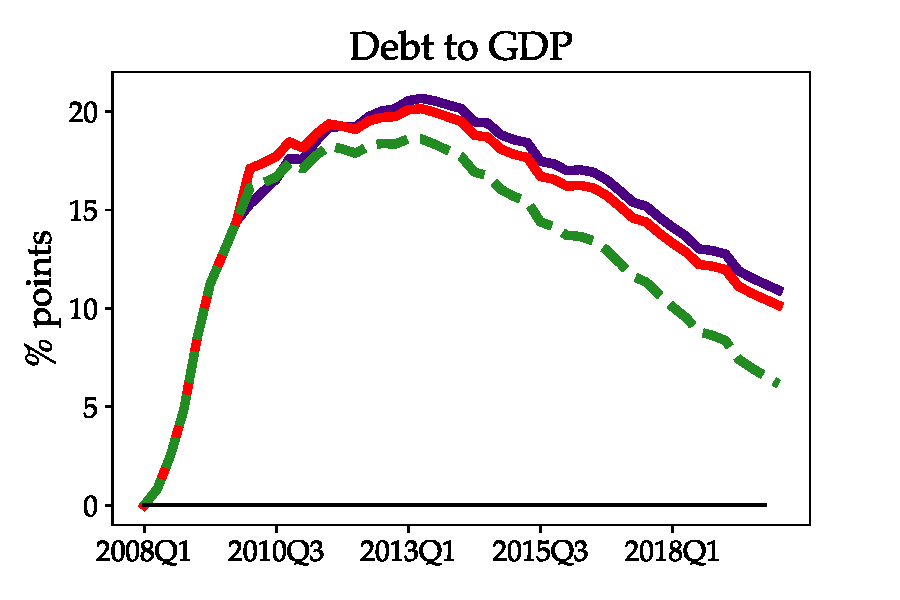
\includegraphics[scale=.57]{text/chapter1/Figures/Fiscal_Consolidation_CounterFactual/debt2GDP_CounterFactual_Fiscal_Consolidation}
\label{fig:c}
\end{minipage}\hspace*{\fill}
\begin{minipage}{0.51\textwidth}
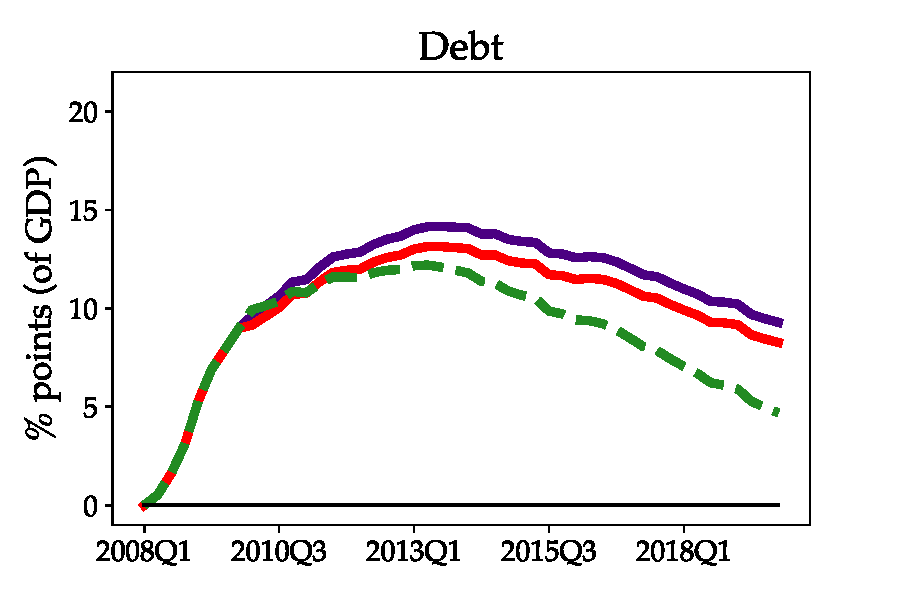
\includegraphics[scale=.57]{text/chapter1/Figures/Fiscal_Consolidation_CounterFactual/debt_CounterFactual_Fiscal_Consolidation}
 \label{fig:d}
\end{minipage}
\medskip
\begin{minipage}{0.51\textwidth}
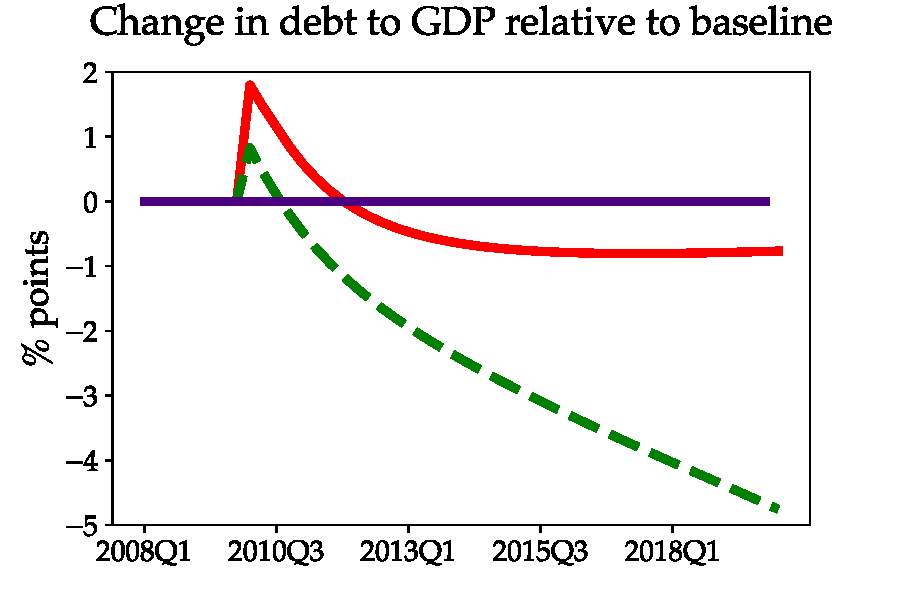
\includegraphics[scale=.57]{text/chapter1/Figures/Fiscal_Consolidation_CounterFactual/change_in_debt2GDP_CounterFactual_Fiscal_Consolidation}
\label{fig:c}
\end{minipage}\hspace*{\fill}
\begin{minipage}{0.51\textwidth}
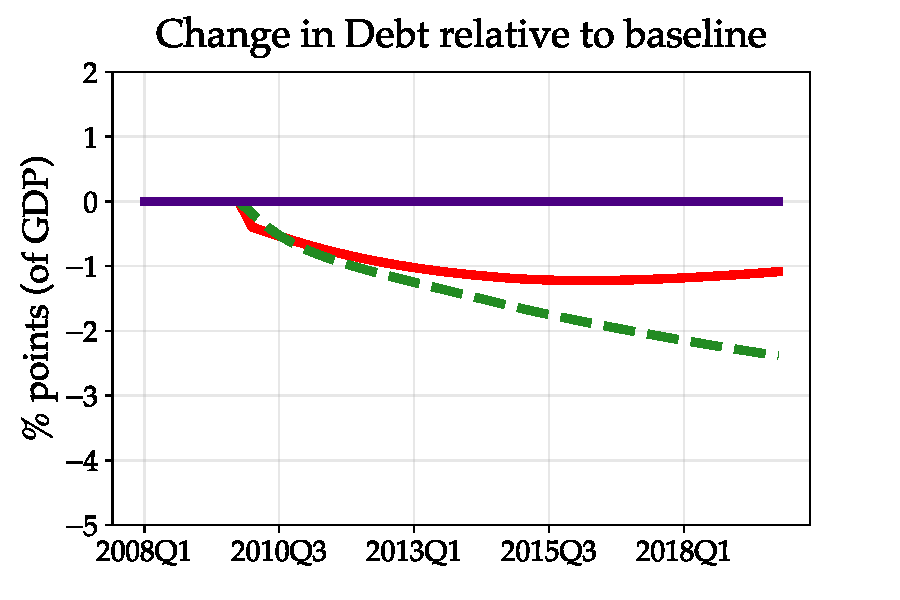
\includegraphics[scale=.57]{text/chapter1/Figures/Fiscal_Consolidation_CounterFactual/change_in_debt_CounterFactual_Fiscal_Consolidation}
 \label{fig:d}
\end{minipage}

\caption{Counterfactual: Fiscal Consolidation in the US}
\floatfoot{Note: This exercise plots the simulated paths of of macro aggregates during the Great Recession from figure \ref{NonTarget} with a fiscal consolidation shock that begins in 2010Q1 under the baseline model and the model without scarring.}

\label{FC_US}
\end{figure}


\hypertarget{Fiscal Consolidation and the Zero Lower Bound}{}
\subsection{Fiscal Consolidation and the Zero Lower Bound}

What are the effects of the zero lower bound on the counterfactual fiscal consolidation in section 7.3? To do so, I redo the experiment in section 7.3 but allow for an active Taylor rule. In particular, I set the Taylor rule coefficient on output, $\phi_{Y}$, to $1/12$ and the Taylor rule coefficient on inflation, $\phi_{\pi}$, to $1.5$.  Further, to illustrate the effect of an aggressive monetary authority, I also perform this experiment again with $\phi_{Y} = 0.2$ Figure \ref{FC_US_no_ZLB} plots the fiscal consolidation exercise with and without the zero lower bound under the baseline Taylor rule and the more aggressive Taylor rule. Without the zero lower bound, fiscal consolidation becomes significantly more effective at reducing debt to GDP. The dashed blue and orange lines demonstrates that the decline in debt to GDP is substantially larger without the zero lower bound. The increased effectiveness of fiscal consolidation in reducing debt to GDP in the absence of the zero lower bound stems from decreasing the cost of debt. Decreasing the interest rate alleviates the fiscal authority's cost of borrowing, and therefore decreases the upward pressure that lost tax revenues place on debt. 


\begin{figure}[t!] % "[t!]" placement specifier just for this example
\centering
\begin{minipage}{0.51\textwidth}
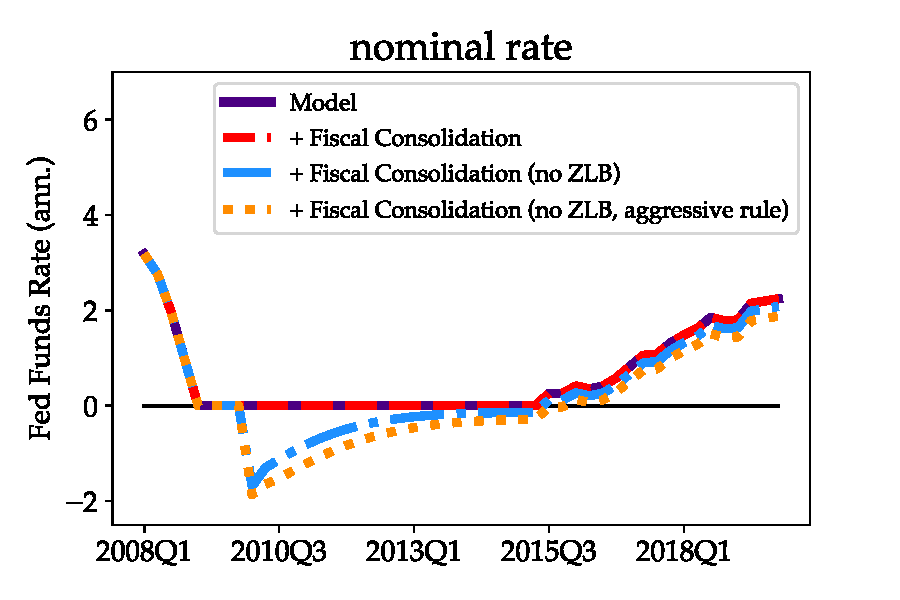
\includegraphics[scale=.57]{text/chapter1/Figures/Fiscal_Consolidation_CounterFactual/FedFunds_FC_no_ZLB_lower}
 \label{fig:a}
\end{minipage}\hspace*{\fill}
\begin{minipage}{0.51\textwidth}
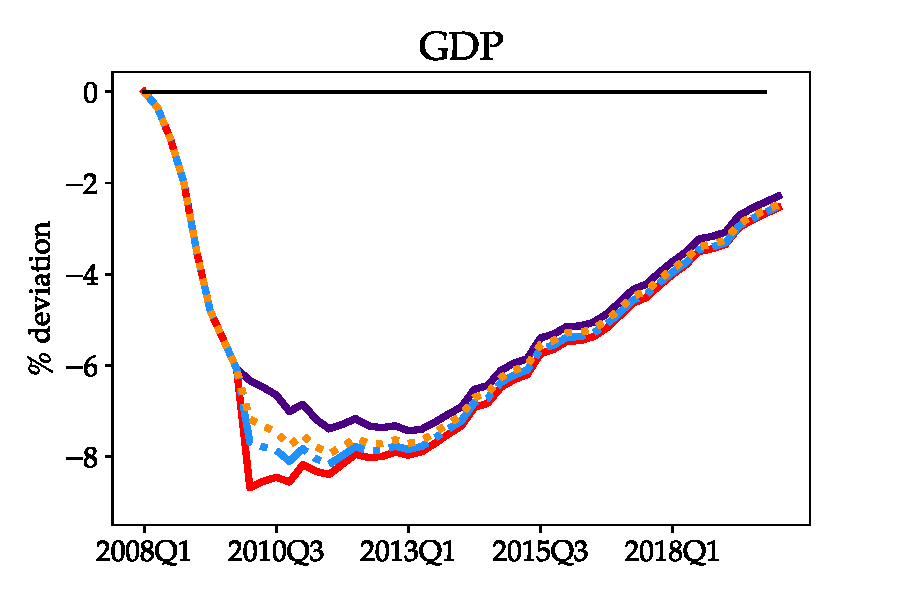
\includegraphics[scale=.57]{text/chapter1/Figures/Fiscal_Consolidation_CounterFactual/GDP_CounterFactual_Fiscal_Consolidation_no_ZLB_lower}
 \label{fig:b}
\end{minipage}

\medskip
\begin{minipage}{0.51\textwidth}
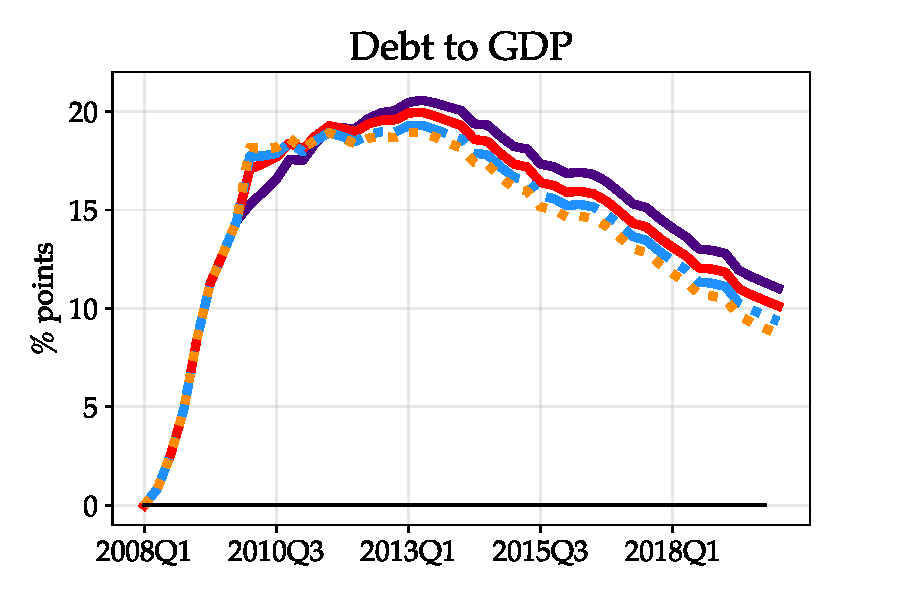
\includegraphics[scale=.57]{text/chapter1/Figures/Fiscal_Consolidation_CounterFactual/debt2GDP_CounterFactual_Fiscal_Consolidation_no_ZLB_lower}
\label{fig:c}
\end{minipage}\hspace*{\fill}
\begin{minipage}{0.51\textwidth}
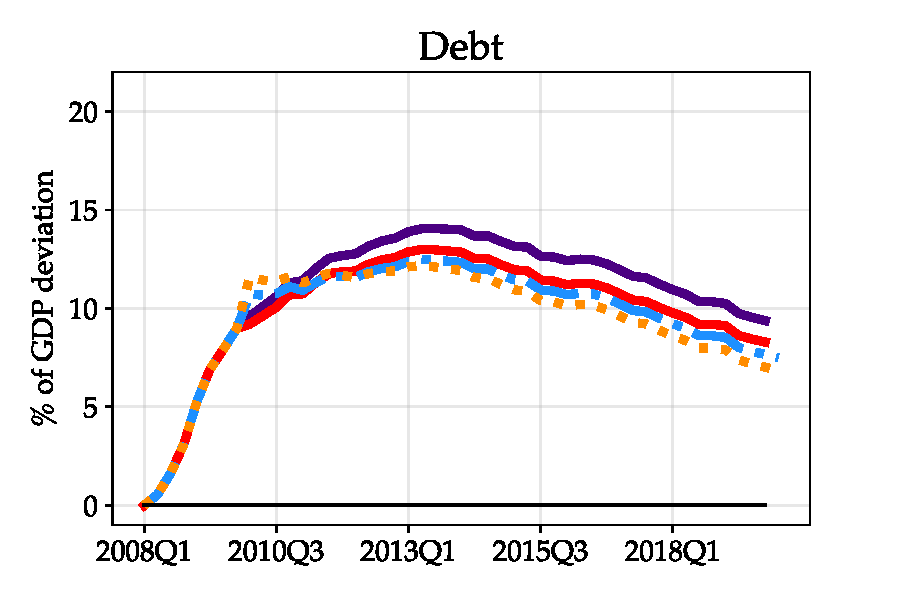
\includegraphics[scale=.57]{text/chapter1/Figures/Fiscal_Consolidation_CounterFactual/debt_CounterFactual_Fiscal_Consolidation_no_ZLB_lower}
 \label{fig:d}
\end{minipage}

\medskip
\begin{minipage}{0.51\textwidth}
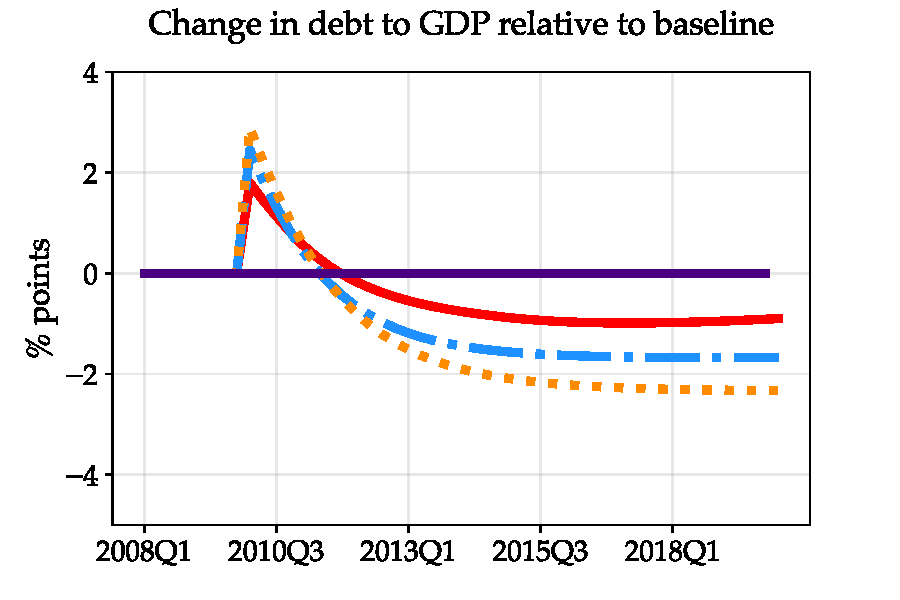
\includegraphics[scale=.57]{text/chapter1/Figures/Fiscal_Consolidation_CounterFactual/change_in_debt2GDP_CounterFactual_Fiscal_Consolidation_no_ZLB}
\label{fig:c}
\end{minipage}\hspace*{\fill}
\begin{minipage}{0.51\textwidth}
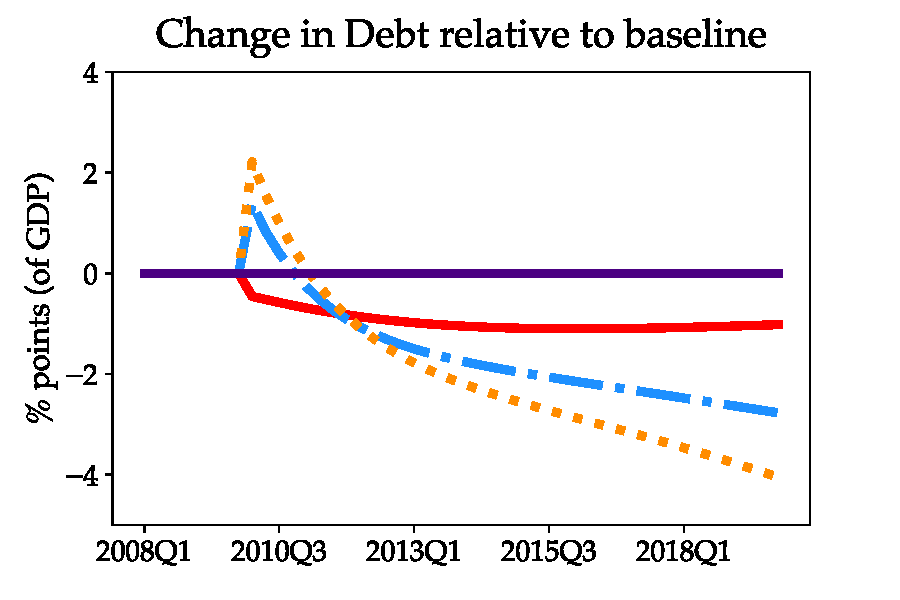
\includegraphics[scale=.57]{text/chapter1/Figures/Fiscal_Consolidation_CounterFactual/change_in_debt_CounterFactual_Fiscal_Consolidation_no_ZLB}
 \label{fig:d}
\end{minipage}


\caption{Counterfactual: Fiscal Consolidation in the US and the effects of the zero lower bound}
\label{FC_US_no_ZLB}
\end{figure}






